\documentclass{standalone}
\usepackage{tikz}
\usepackage{xinttools}

\usetikzlibrary{calc,math}



\begin{document}

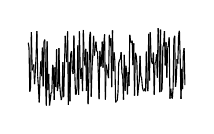
\begin{tikzpicture}
  \foreach \i in {1,...,200} {
    \tikzmath{
      real \x;
      real \y;
      \x = \i / 100;
      \y = random();
    }
    \coordinate (P\i) at (\x,\y);
  }

  \foreach \i in {1,...,199} {
    \tikzmath{
      int \j;
      \j = int(\i + 1);
    }
    \draw (P\i) -- (P\j);
  }
\end{tikzpicture}

\end{document}
